

\subsubsection{Tavola dei Volumi}

\noindent\makebox[\textwidth]{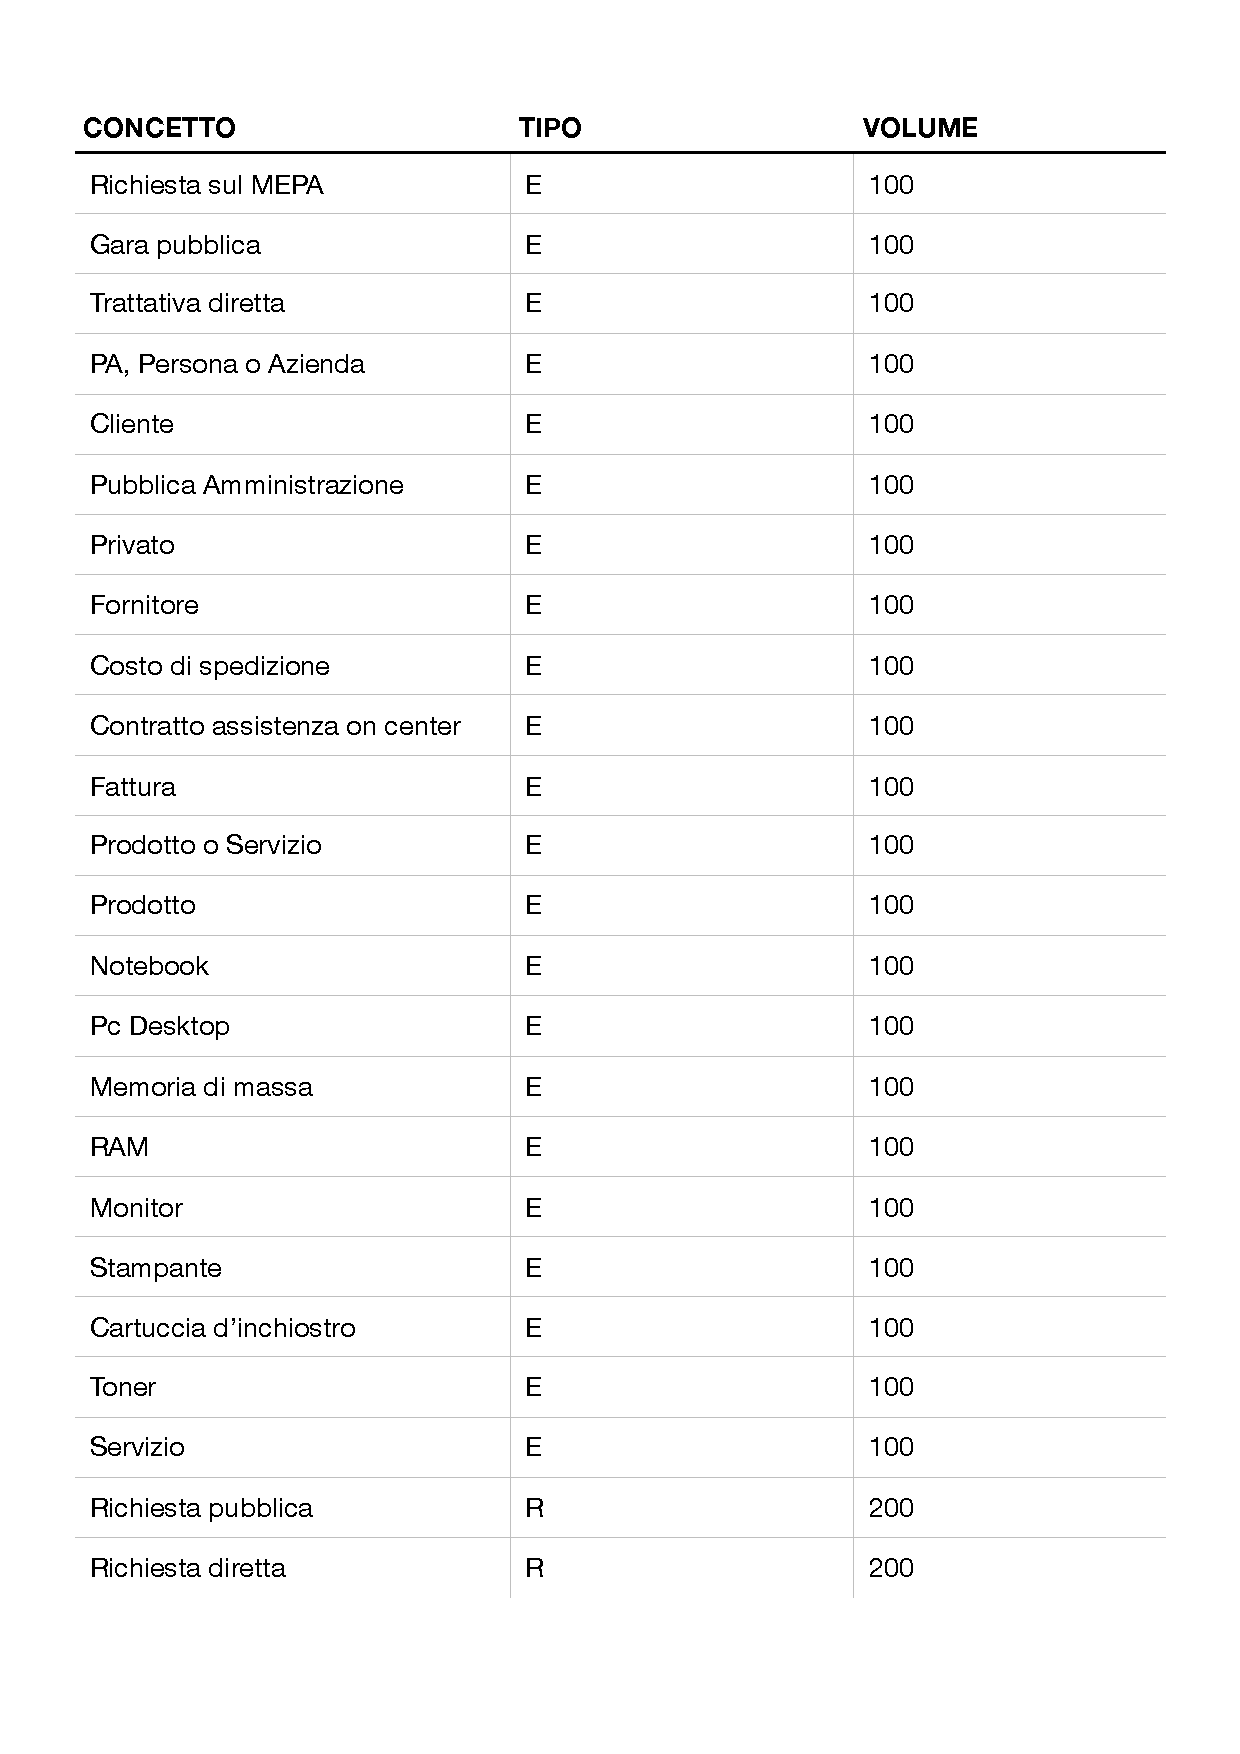
\includegraphics[page=1, width=\textwidth+1.5cm]{./pdf/tavola_volumi.pdf}}
\newpage
\noindent\makebox[\textwidth]{\includegraphics[page=2, width=\textwidth+1.5cm, trim=0 16cm 0 0]{./pdf/tavola_volumi.pdf}}

\noindent
Abbiamo stimato che la base di dati ha un ciclo di vita di 5 anni.
\newline
Abbiamo considerato che in un anno ci sono 280 giorni di lavoro, e di conseguenza circa 46 settimane di lavoro.
\newline
Si è stimato che ogni contratto di assistenza on center comprende mediamente 3 servizi erogati.
\newline
Abbiamo stimato che ogni richiesta del Mepa ha mediamente 3 descrizioni richieste diverse.
\newline
Mediamente ogni fornitore ha 4 costi di spedizione diversi, e abbiamo tenuto conto del fatto che alcuni fornitori possono avere alcuni costi di spedizione identici.
\newline
Per il catalogo, che contiene i prezzi di vendita dei prodotti dei singoli fornitori, abbiamo ritenuto che ogni fornitore non venderà tutti i prodotti presenti nel nostro database, il valore 10000 è quindi un'approssimazione nata da questa considerazione.
\newline
Facciamo notare che le spedizioni sono considerate solo per le stipulazioni d'acquisto, perchè l'azienda opera in dropshipping e quindi spedisce direttamente al cliente tramite accordi con i fornitori.

\subsubsection{Tavola delle Operazioni}

\noindent\makebox[\textwidth]{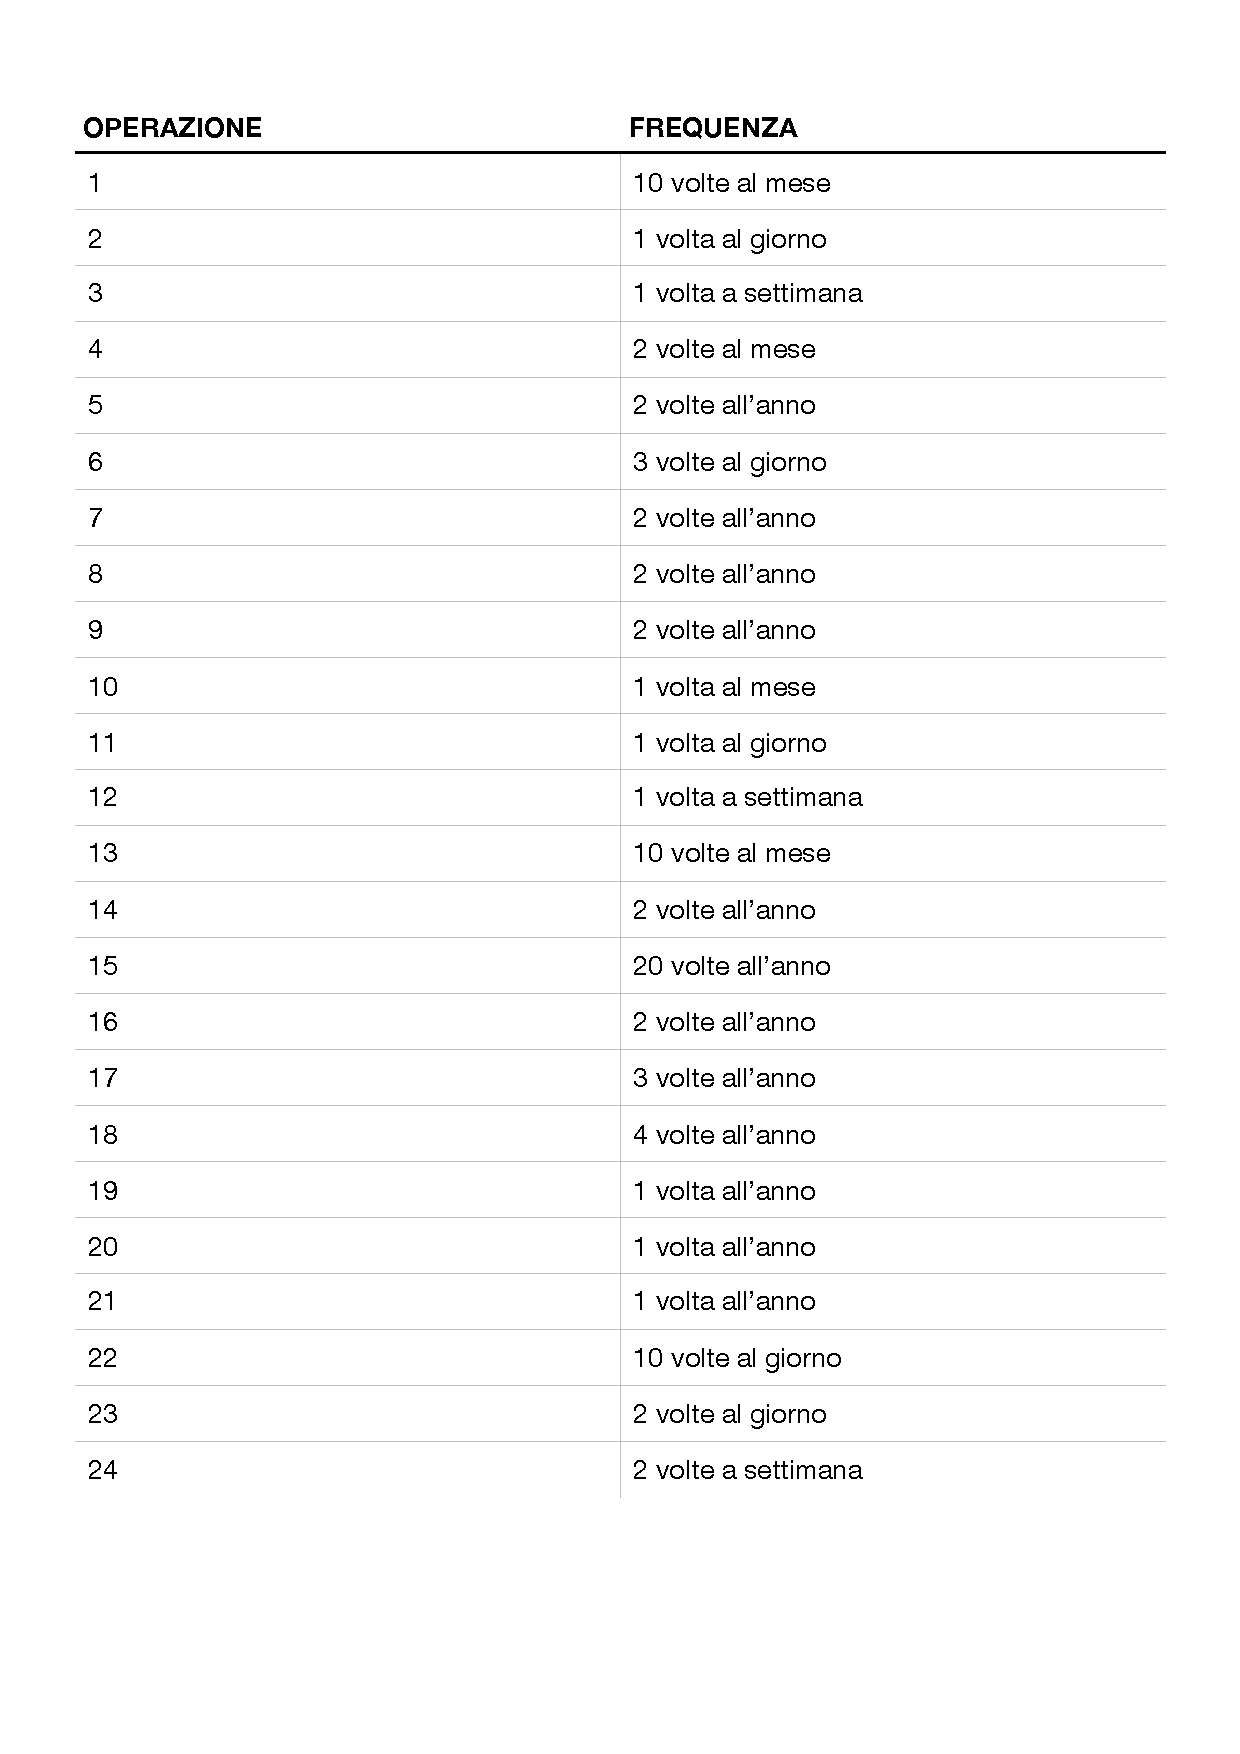
\includegraphics[page=1, width=\textwidth+1.5cm]{./pdf/tavola_operazioni.pdf}}
\newpage
\noindent\makebox[\textwidth]{\includegraphics[page=2, width=\textwidth+1.5cm]{./pdf/tavola_operazioni.pdf}}
